

\subsection{System setup}
\label{subsec:setup}

\begin{figure*}[t]
    \centering
    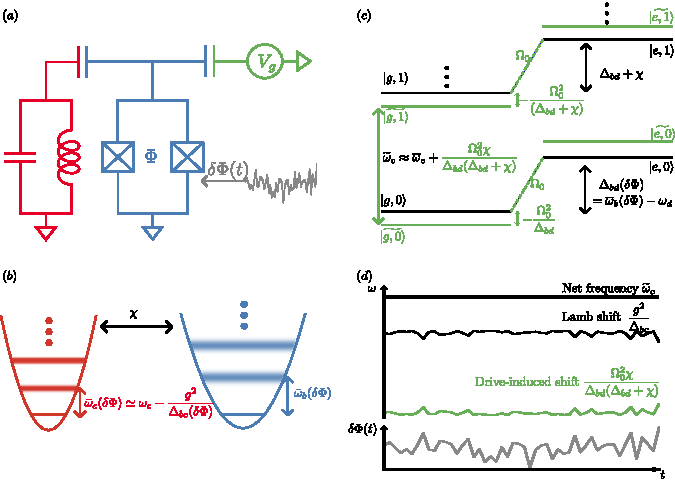
\includegraphics[width=\textwidth]{plot/device_plot/deviceplot/device.pdf}
    \caption[Scheme for engineering a cavity frequency at a driven sweet spot.]{
\textbf{Scheme for engineering a cavity frequency at a driven sweet spot.}
\textbf{(a)} Circuit schematic of a flux-tunable transmon (FTT) dispersively coupled to a superconducting cavity and driven by a coherent voltage source $V_g$. Flux noise $\delta\Phi(t)$ modulates the FTT frequency and provides the dominant noise channel.
\textbf{(b)} Noise transduction via the Lamb shift. The bare modes have frequencies $\omega_c$ and $\omega_b(\delta\Phi)$ with flux-dependent detuning $\Delta_{bc}(\delta\Phi)=\omega_b(\delta\Phi)-\omega_c$. The coupling $g$ hybridizes the modes, yielding dressed frequencies $\bar{\omega}_{b/c}(\delta\Phi)$; the cavity frequency acquires a Lamb shift $-g^2/\Delta_{bc}$ and therefore inherits sensitivity to $\delta\Phi(t)$.
\textbf{(c)} Drive-induced, photon-number--dependent shift in the frame rotating at $\omega_d$. A coherent drive of amplitude $\Omega_0$ hybridizes the manifolds $|{g,m}\rangle$ and $|{e,m}\rangle$, producing level repulsion (green) that renormalizes the cavity transition frequency in an $m$-dependent manner.
\textbf{(d)} First-order noise cancellation at the driven sweet spot. In the presence of $\delta\Phi(t)$ (gray), the static Lamb-shift contribution to the cavity frequency (black) is compensated by the drive-induced shift (green) at an appropriate drive, yielding a net cavity frequency $\tilde{\omega}_c$ (thick black) that is first-order insensitive to flux fluctuations (a flux-insensitive point in the sense of vanishing first-order susceptibility).
}
    \label{fig:device}
\end{figure*}

The Hamiltonian of the FTT--cavity system is
\begin{align}
H(t) &= H_{\mathrm{static}} + H_{\mathrm{noise}}, \label{H}\\
H_{\mathrm{static}} &=
\omega_b\, b^\dagger b
+ \frac{K}{2}\, b^{\dagger 2} b^{2}
+ \omega_c\, c^\dagger c
+ g\,(b+b^\dagger)(c+c^\dagger), \label{Hstatic}\\
H_{\mathrm{noise}} &= \delta\omega_b(t)\, b^\dagger b .
\end{align}
Here, $b$ ($c$) annihilates an excitation in the FTT (cavity) mode; $K$ is the FTT anharmonicity; and $g$ is the coupling strength. Flux noise can cause both depolarization and dephasing. Considering flux noise as small-amplitude $1/f$ noise, we neglect depolarization at GHz-frequency transitions triggered (see Appendix~\ref{app:hamiltonian-derivation-noise} for more details). Thus, the noise dominantly causes an FTT-frequency fluctuation $\delta\omega_b(t)=\delta\Phi(t)\,\partial\omega_b/\partial\Phi$, where $\Phi$ is the static flux bias and $\delta\Phi(t)$ is its fluctuation.

In the dispersive frame \cite{Blais2021}, the effective Hamiltonian for $H_\text{static}$ takes the form
\begin{align}
\label{Hdisp}
H_\text{disp} =
\bar{\omega}_b\, b^\dagger b
+ \frac{K}{2}\, b^{\dagger 2} b^{2}
+ \bar{\omega}_c\, c^\dagger c
+ \chi\, b^\dagger b\, c^\dagger c,
\end{align}
where $\chi$ is the dispersive shift and $\bar{\omega}_b$ and $\bar{\omega}_c$ are the Lamb-shifted FTT and cavity frequencies, which depend on the detuning $\Delta_{bc}=\omega_b-\omega_c$:
\begin{align}
\chi &\approx 2\frac{g^2}{\Delta_{bc}^2}K,\quad
\bar{\omega}_b \approx \omega_b + \frac{g^2}{\Delta_{bc}}, \quad
\bar{\omega}_c \approx \omega_c - \frac{g^2}{\Delta_{bc}}.
\end{align}
The noise Hamiltonian $H_{\mathrm{noise}}$ primarily induces dephasing between eigenstates of $H_\text{disp}$ (see Appendix~\ref{Hnoise_transfer}). In particular, because $\Delta_{bc}$ depends on $\bar{\omega}_c$, FTT-frequency fluctuations $\delta\omega_b(t)$ lead to cavity-frequency fluctuations
\begin{align}
\delta\bar{\omega}_c(t)
= \frac{\partial \bar{\omega}_c}{\partial \omega_b}\,\delta\omega_b(t)
\approx \frac{g^2}{\Delta_{bc}^2}\,\delta\omega_b(t),
\end{align}
thereby producing cavity dephasing. This is summarized in Fig.~\ref{fig:device}(b).